% $Id$
%

\section{Bootstrap}


%%---------------------------------------------------------------

\begin{frame}
\frametitle{¿Qué es Bootstrap?}

\begin{itemize}
  \item Bootstrap es un framework libre para desarrollo web
  \item Realizado por ingenieros de Twitter
  \item Incluye plantillas HTML y CSS con tipografías, formas, botones, cuadros, barras de navegación, carruseles de imágenes y muchas otras
  \item También existe la posibilidad de utilizar plugins de JavaScript
  \item Aunque su preferencia es \emph{mobile first}, permite crear diseños que se ven bien en múltiples dispositivos (\emph{responsive design})
\end{itemize}

\end{frame}

%%---------------------------------------------------------------

\begin{frame}
\frametitle{Ventajas de Bootstrap (para ingenieros)}

\begin{itemize}
  \item Es sencillo y rápido
  \item Se adapta a distintos dispositivos (\emph{responsive design})
  \item Proporciona un diseño consistente
  \item Es compatible con los navegadores modernos
  \item Es software libre
\end{itemize}

\end{frame}

%%---------------------------------------------------------------

\begin{frame}[fragile]
\frametitle{Ficheros de Bootstrap}

\begin{itemize}
  \item Se pueden descargar y servir como cualquier otro fichero estático
  \item O se pueden referenciar desde un CDN
  \begin{itemize}
    \item CDN: Content Delivery Network
  \end{itemize}
  \item Con un CDN (Content Delivery Network) no hace falta tener Bootstrap en nuestros
archivos. Además, si un usuario ya ha descargado esas URLs, probablemente
las tenga ya en la caché del navegador (con el consiguiente ahorro de tiempo).
\end{itemize}


\end{frame}


%%---------------------------------------------------------------
%
%\begin{frame}[fragile]
%\frametitle{Ficheros de Bootstrap}
%
%\begin{footnotesize}
%\begin{verbatim}
%bootstrap/
%|--- css/
%|   |--- bootstrap.css
%|   |--- bootstrap.css.map
%|   |--- bootstrap.min.css
%|   |--- bootstrap-theme.css
%|   |--- bootstrap-theme.css.map
%|   |--- bootstrap-theme.min.css
%|--- js/
%|   |--- bootstrap.js
%|   |--- bootstrap.min.js
%|--- fonts/
%    |--- glyphicons-halflings-regular.eot
%    |--- glyphicons-halflings-regular.svg
%    |--- glyphicons-halflings-regular.ttf
%    |--- glyphicons-halflings-regular.woff
%    |--- glyphicons-halflings-regular.woff2
%\end{verbatim}
%\end{footnotesize}
%
%\end{frame}


%%---------------------------------------------------------------

\begin{frame}[fragile]
\frametitle{La plantilla de Bootstrap}


\begin{footnotesize}
\begin{verbatim}
<!doctype html>
<html lang="en">
  <head>
    <!-- Required meta tags -->
    <meta charset="utf-8">
    <meta name="viewport" content="width=device-width, initial-scale=1">

    <!-- Bootstrap CSS -->
    <link href="https://cdn.jsdelivr.net/npm/bootstrap@5.0.0/dist/css/bootstrap.min.css" rel="stylesheet" integrity="sha384-wEmeIV1mKuiNpC+IOBjI7aAzPcEZeedi5yW5f2yOq55WWLwNGmvvx4Um1vskeMj0" crossorigin="anonymous">

    <title>Hello, world!</title>
  </head>
  <body>
      <h1>Hello, world!</h1>

    <!-- Option 1: Bootstrap Bundle with Popper -->
    <script src="https://cdn.jsdelivr.net/npm/bootstrap@5.0.0/dist/js/bootstrap.bundle.min.js" integrity="sha384-p34f1UUtsS3wqzfto5wAAmdvj+osOnFyQFpp4Ua3gs/ZVWx6oOypYoCJhGGScy+8" crossorigin="anonymous"></script>
</html>
\end{verbatim}
\end{footnotesize}

\end{frame}



%%---------------------------------------------------------------
%
%\begin{frame}[fragile]
%\frametitle{Bootstrap en CDN}
%
%\begin{itemize}
%  \item Con un CDN (Content Delivery Network) no hace falta tener Bootstrap en nuestros
%archivos. Además, si un usuario ya ha descargado esas URLs, probablemente
%las tenga ya en la caché del navegador (con el consiguiente ahorro de tiempo).
%\end{itemize}

%\begin{footnotesize}
%\begin{verbatim}
% <!-- Latest compiled and minified CSS -->
%<link rel="stylesheet" 
%href="http://maxcdn.bootstrapcdn.com/bootstrap/3.3.7/css/bootstrap.min.css">
%
%<!-- jQuery library -->
%<script 
% src="https://ajax.googleapis.com/ajax/libs/jquery/1.11.1/jquery.min.js">
%</script>
%
%<!-- Latest compiled JavaScript -->
%<script 
% src="http://maxcdn.bootstrapcdn.com/bootstrap/3.3.7/js/bootstrap.min.js">
%</script>
%\end{verbatim}
%\end{footnotesize}
%
%
%\end{frame}


%%---------------------------------------------------------------

\begin{frame}[fragile]
\frametitle{Mobile first}

% Info: https://developer.mozilla.org/es/docs/M%C3%B3vil/Viewport_meta_tag

\begin{itemize}
  \item En los navegadores, el \emph{viewport} es la parte visible de un documento
  \item Si el documento es mayor que el área de visualización, el usuario puede cambiar la vista desplazándose
  \item Con una propiedad de etiqueta meta, podemos indicar la escala inicial del \emph{viewport}
\end{itemize}

\begin{footnotesize}
\begin{verbatim}
<meta name="viewport" content="width=device-width, initial-scale=1">
\end{verbatim}
\end{footnotesize}

\begin{itemize}
  \item Se puede inhabilitar el zoom en dispositivos móviles con \texttt{user-scalable=no}
  \item Los usuarios sólo podrán hacer \emph{scroll} y tendrá una apariencia nativa.
  \item Usar con precaución. No vale para todas las aplicaciones
\end{itemize}

\begin{footnotesize}
\begin{verbatim}
<meta name="viewport" content="width=device-width, initial-scale=1, 
maximum-scale=1, user-scalable=no">
\end{verbatim}
\end{footnotesize}

\end{frame}


%%---------------------------------------------------------------

\begin{frame}[fragile]
\frametitle{Contenedores}

\begin{itemize}
   \item Bootstrap requiere tener un elemento contenedor que cubra contenidos y el sistema de rejilla.
   \item Para un contenedor responsivo de tamaño fijo, usa \texttt{.container}
\end{itemize}

\begin{footnotesize}
\begin{verbatim}
<div class="container">
  ...
</div>
\end{verbatim}
\end{footnotesize}

\begin{itemize}
  \item Si se desea un contenedor con el ancho total (del \emph{viewport}), se ha de usar \texttt{.container-fluid}
\end{itemize}

\begin{footnotesize}
\begin{verbatim}
<div class="container-fluid">
  ...
</div>
\end{verbatim}
\end{footnotesize}

\end{frame}



%%---------------------------------------------------------------

\begin{frame}
\frametitle{El sistema de rejilla (I)}

El diseño de páginas basado en rejilla se realiza mediante filas y
columnas donde se colocan los contenidos. Así funciona la rejilla de Bootstrap:

\begin{itemize}

  \item Filas, dentro un contenedor, agrupan horizontalmente varias columnas, que son las que tienen contenido
  \item La pantalla se divide en 12 columnas
  \item Las columnas definen su anchura especificando cuántas columnas de la fila ocupan
  \item Hay clases CSS (como por ejemplo .row y .col-xs-4) para crear rejillas rápidamente
  \item Hay padding entre columnas. En la primera y última columnas, las filas (elementos .row) aplican márgenes negativos

\end{itemize}

\end{frame}

%%---------------------------------------------------------------

\begin{frame}[fragile]
\frametitle{El sistema de rejilla (y II)}

% Ejemplos: http://getbootstrap.com/examples/grid/

\begin{center}
\begin{figure}[p]
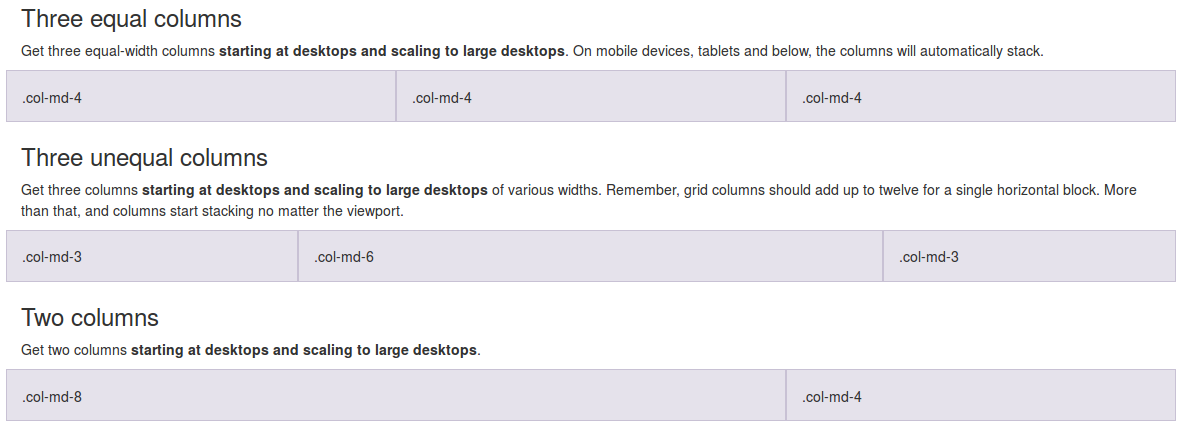
\includegraphics[width=0.99\textwidth]{figs/grid.png}
\end{figure}
\end{center}

\end{frame}



%%---------------------------------------------------------------

\begin{frame}[fragile]
\frametitle{Responsive design}

\begin{center}
\begin{figure}[p]
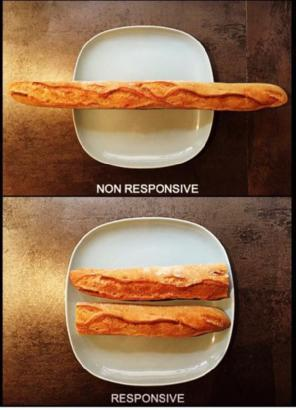
\includegraphics[width=0.99\textwidth]{figs/responsive.jpg}
\end{figure}
\end{center}

\begin{flushright}
{\tiny
Source: https://image-store.slidesharecdn.com/420d15aa-cbf0-4ded-ac42-fcf728610bc1-original.jpeg
}
\end{flushright}

\end{frame}



%%---------------------------------------------------------------

\begin{frame}[fragile]
\frametitle{Responsive design en Bootstrap}

Móviles y escritorio:

\begin{center}
\begin{figure}[p]
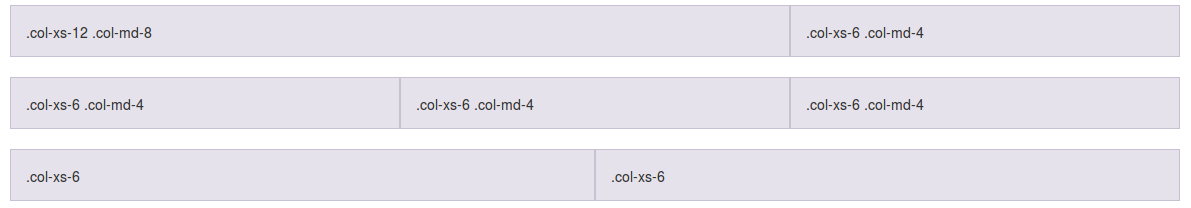
\includegraphics[width=0.99\textwidth]{figs/grid-responsive.png}
\end{figure}
\end{center}

Móvil, tableta y escritorio:

\begin{center}
\begin{figure}[p]
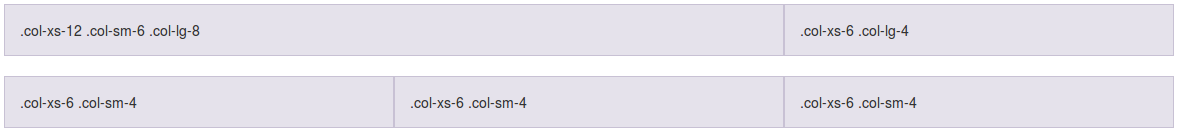
\includegraphics[width=0.99\textwidth]{figs/grid-responsive2.png}
\end{figure}
\end{center}

\end{frame}



%%---------------------------------------------------------------

\begin{frame}[fragile]
\frametitle{Breakpoints}

Bootstrap incluye seis puntos de interrupción predeterminados, a veces denominados niveles de cuadrícula, para construir de manera \emph{responsive}:

\begin{table}[]
\begin{tabular}{lcc}

{\bf Breakpoint} & {\bf Class infix} &  {\bf Dimensions} \\ \hline
X-Small & None & $<576px$ \\
Small & sm & $>=576px$ \\
Medium & md & $>=768px$ \\
Large & lg & $>=992px$ \\
Extra large & xl & $>=1200px$ \\
Extra extra large & xxl & $>=1400px$
\end{tabular}
\end{table}


\end{frame}



%%---------------------------------------------------------------

%\begin{frame}
%\frametitle{Otras clases}

%Bootstrap viene con una serie de estilos (generalmente en formato de clase CSS)
%por defecto, entre otros:

%\begin{itemize}
%  \item \texttt{table}
%  \item \texttt{form}
%  \item \texttt{buttons}
%  \item \texttt{img-responsive}
%  \item \texttt{helper} classes
%  \item y otras utilidades responsivas
%\end{itemize}

%\end{frame}


%%---------------------------------------------------------------

%\begin{frame}
%\frametitle{JavaScript}

%Con Bootstrap vienen una serie de \emph{plug-ins} de JavaScript, como:

%\begin{itemize}
%  \item transitions.js: efectos de transición
%  \item modal.js: diálogos simples y flexibles
%  \item dropdown.js: menús desplegables
%  \item scrollspy.js: según vamos bajando en la página, actualiza la \emph{navbar}
%  \item tab.js: pestañas
%  \item tooltip.js y popover.js: cajas con consejos o más información
%  \item alert.js: alertas
%  \item button.js: botones
%  \item collapse.js: permite mostrar/ocultar elementos
%  \item carousel.js: el (ya famoso carrusel)
%  \item affix.js: Menú de navegación lateral
%\end{itemize}

%\end{frame}


%%---------------------------------------------------------------

%\begin{frame}
%\frametitle{Bootlint}

%\begin{itemize}
%  \item Herramienta que detecta algunos errores comunes el HTML de diseños \texttt{Bootstrap}
%  \item Comprueba que las instancias de componentes Bootstrap han sido correctamente estructurados
%  \item Analiza también la inclusión de ciertas etiquetas $<meta>$, la declaración DOCTYPE HTML5, etc.
%  \item Página web: \url{https://github.com/twbs/bootlint}
%\end{itemize}

%\end{frame}

%%---------------------------------------------------------------

\begin{frame}
\frametitle{Otros sitios de interés}



\begin{itemize}
  \item Listado de recursos sobre Bootstrap \\
        \url{http://bootsnipp.com/resources}
  \item Bootsnipp: Cientos de componentes adicionales \\
        \url{http://www.bootsnipp.com}
  \item Startboostrap: Plantillas y temas Bootstrap (gratis) \\
        \url{http://startbootstrap.com/}  
  \item WrapBoostrap: Plantillas y temas Boostrap (de pago) \\
        \url{https://wrapbootstrap.com/}
  \item BootTheme: Generador (no libre) de diseños Bootstrap \\
        \url{http://www.boottheme.com/}
\end{itemize}

\end{frame}


